\clearpage
\section{MISO output drive experiment: 15 November 2026}
The routed diagnostic checkpoint was reused without synthesis, placement or
routing changes. Only HMISO (F24, bank 14, LVCMOS33) DRIVE was changed from
12 to 4 mA. SLEW remained SLOW. Both images retain RTL ID
\texttt{30096dcc}; bitstream hashes distinguish the electrical variants.
The 4 mA variant meets timing (setup slack 0.019 ns, hold slack 0.061 ns).

The FPGA setting affects the FPGA-to-buffer segment. On PM12 schematic sheet 4,
HMISO drives DD29 (SN74LVC1G17DBV, 3.3 V), followed by R132 (47 ohm) and
HDMI PM\_SPI\_MISO. DD29 remains the cable driver. Consequently this experiment
cannot directly reduce the cable driver's configured strength.
The voltage standard remains 3.3 V; DRIVE is not a constant-current limit.

The protocol compares 12 mA, 4 mA, then 12 mA again, with normal parser operation
and no MISO clamp. All stimulus replies are checked. The observer independently
records SYS reset and MMCM LOCK. External clock configuration, Kasli output
directions and buffer enables are retained throughout. The original diagnostic image \texttt{c7531465} is restored at completion.

\begin{center}
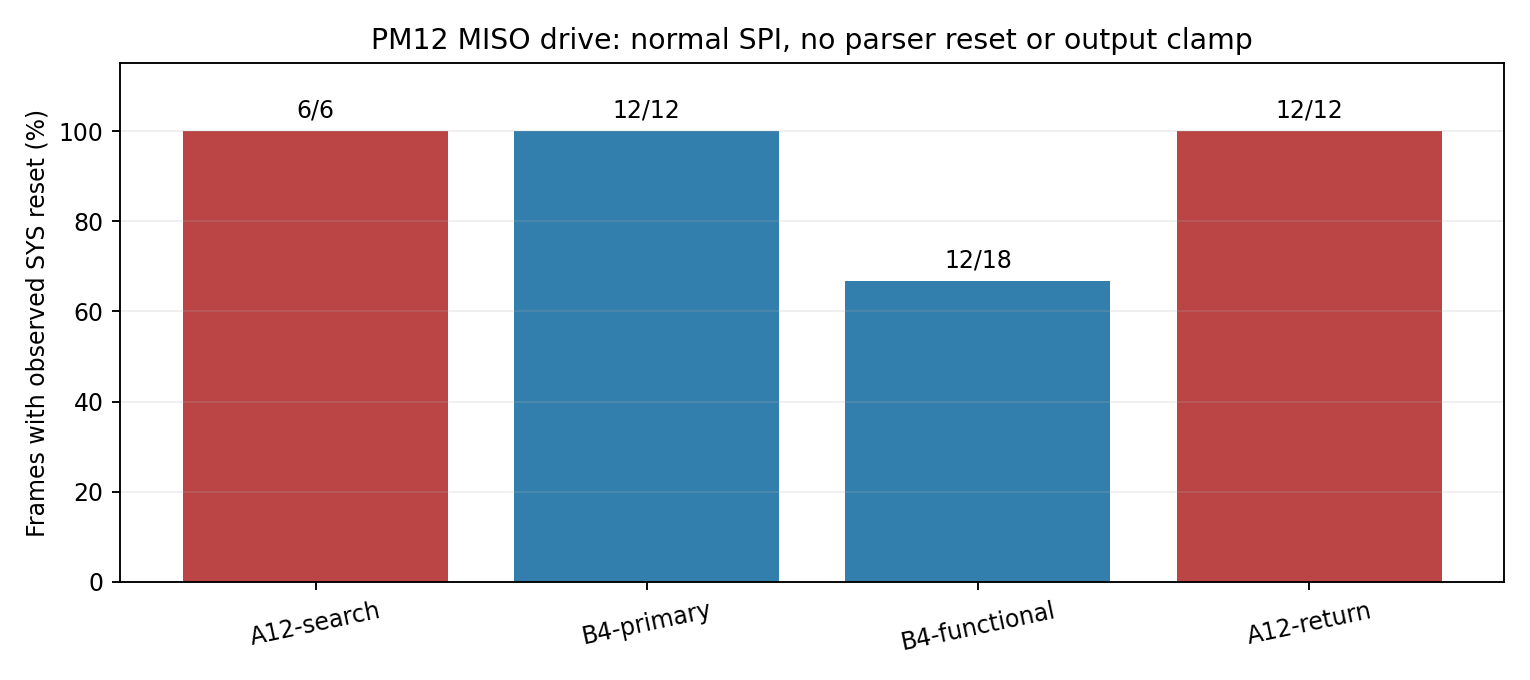
\includegraphics[width=\linewidth]{miso-drive.png}
\end{center}

\begin{center}\begin{tabular}{lrr}\toprule
Condition & SYS resets / frames & Bad SPI replies\\\midrule
12 mA: initial control, divider 601/read 0 &6/6&0\\
4 mA: matched primary test &12/12&0\\
4 mA: additional reads 0--2, dividers 601/61 &12/18&0\\
12 mA: return control, divider 601/read 0 &12/12&0\\\bottomrule
\end{tabular}\end{center}
The lower FPGA drive did not suppress resets. In the additional readout checks,
reads 0 and 1 produced resets, while read 2 remained quiet at both dividers.
The identical primary failure rate supports retaining the original electrical
configuration. It does not establish the coupling mechanism or rule out an
issue downstream of DD29. Raw capture and load receipts are retained under
\texttt{system/evidence-miso-drive-20261115}.

Restoration completed successfully: frontend readiness was 0xfff, power-good
was healthy, and all twelve physical ADC bank-A captures passed on the first
attempt. Kasli output drivers remained enabled; the original divider was restored.
